




%\section{Qt6 Desktop Applications}
\section{Τι είναι το Qt;}
Το Qt είναι μια δημοφιλής βιβλιοθήκη ανάπτυξης εφαρμογών γραφικής διεπαφής 
χρήστη το οποίο είναι διαθέσιμο σε C++ και Python. Με το Qt
είναι εφικτή η υλοποίηση cross-platform εφαρμογών με το τελικό αποτέλεσμα
να είναι μια αξιοπρεπής διεπαφή χρήστη που λειτουργεί αποτελεσματικά και
αξιόπιστα, υποστηρίζοντας μια πληθώρα συστημάτων όπως Windows, Linux, MacOS, Android και ενσωματωμένα συστήματα. 
Παρακάτω γίνεται περιγραφή της λειτουργίας της βιβλιοθήκης αυτής με χρήση παραδειγμάτων σε γλώσσα προγραμματισμού C++ 
μιας και είναι η γλώσσα στην οποία έχει γραφεί το παρόν πρόγραμμα. Τα παραδείγματα
που θα δούμε αφορούν τα εργαλεία που προσφέρει η βιβλιοθήκη αυτή και συνδυάζονται
από το πρόγραμμα για να παραχθεί το τελικό αποτέλεσμα.



\section{Ένα απλό πρόγραμμα σε Qt6}
Για την δημιουργία ενός παραθύρου Qt6 πρέπει πρώτα να δημιουργηθεί ένα αντικείμενο
τύπου \textbf{QApplication}[1] και στην συνέχεια να αρχικοποιηθεί ένα αντικείμενο 
\textbf{QWidget}[2] το οποίο θα αποτελέσει το παράθυρο της εφαρμογής πάνω στο
οποίο θα προστεθούν τα υπόλοιπα στοιχεία της γραφικής διεπαφής για τις λειτουργίες
του προγράμματος. Παρακάτω βλέπουμε ένα παράδειγμα με την αντίστοιχη περιγραφή
μεταφρασμένη σε κώδικα.

\begin{lstlisting}[language=C++, style=cppstyle]
#include <QApplication>
#include <QWidget>


class MyWidget : public QWidget 
{
public:
    MyWidget(QWidget *parent = nullptr) : QWidget(parent) 
    {
        setFixedSize(400, 300);
        setWindowTitle("P2019140 - Konstantinos Tourtsakis");
    }
};

int main(int argc, char *argv[]) 
{
    QApplication app(argc, argv);

    MyWidget widget;
    widget.show();

    return app.exec();
}

\end{lstlisting}


\begin{figure}[H]
    \centering
    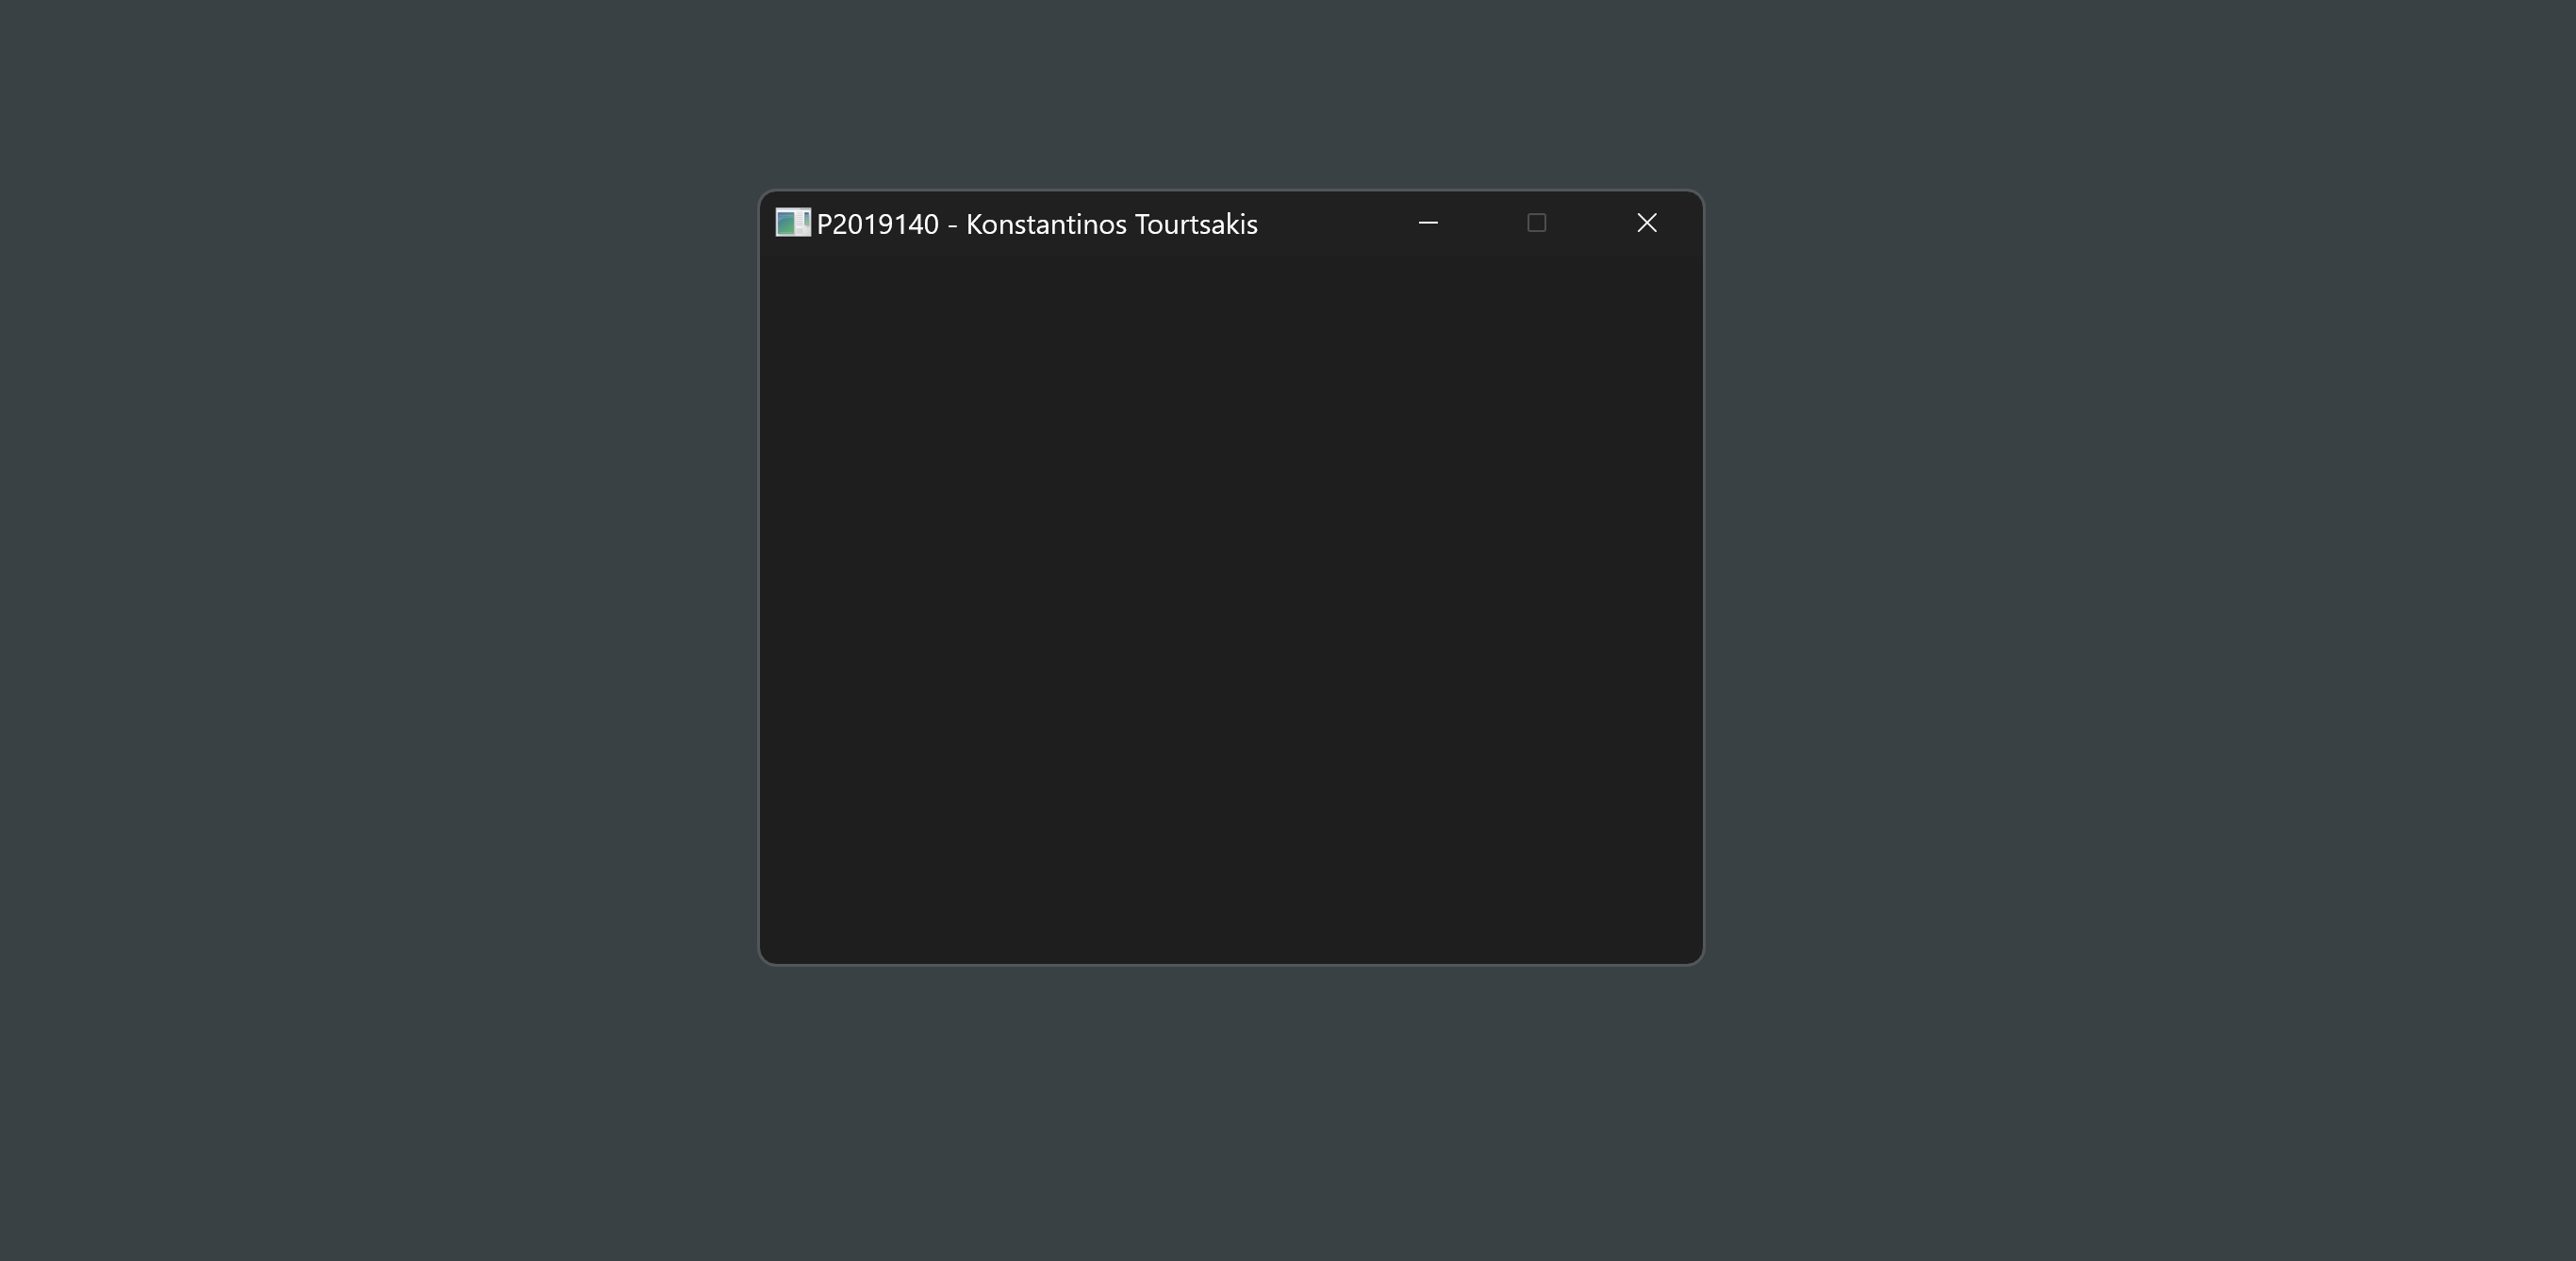
\includegraphics[width=1.0\textwidth]{./images/simple_qt6_app.png}
    \caption{Παράδειγμα Qt6 εφαρμογής}
\end{figure}




Η κλάση MyWidget κληρονομεί την κλάση QWidget. Το παράθυρο το οποίο δημιουργείται
εμφανίζεται στο μέγεθος που ορίστηκε και στην συνέχεια επιστρέφεται το αντικείμενο της εφαρμογής
το οποίο το διαχειρίζεται η βιβλιοθήκη κατά την έξοδο εκτέλεσης του προγράμματος.


\section{Προσθήκη στοιχείων γραφικής διεπαφής σε Qt6}
Κάθε εφαρμογή γραφικής διεπαφής παρέχει στοιχεία μέσω των οποίων γίνεται η διαχείριση
των δεδομένων που επεξεργάζεται και η εκτέλεση των λειτουργιών του. Συνήθως τα δεδομένα αυτά δεν είναι τίποτε άλλο από
τους βασικούς τύπους δεδομένων που υποστηρίζουν οι γλώσσες προγραμματισμού:
int, bool, float και string. Επιπλέον υπάρχουν στοιχεία με τα οποία εξυπηρετείται
αποτελεσματικότερα ο σκοπός του προγράμματος, είτε λόγω ευκολίας είτε για λόγους κατανόησης
από τον χρήστη. Παρακάτω βλέπουμε τα στοιχεία που αξιοποιεί το πρόγραμμα της
εργασίας για την επίτευξη του σκοπού του.

\subsection{Δημιουργία QPushButton}
Ένα QPushButton[3] είναι ένα κουμπί το οποίο έχει την ιδιότητα εκτέλεσης λειτουργιών.
Για την προσθήκη μιας λειτουργίας πάνω στο κουμπί αυτό χρειάζεται να γίνει η
σύνδεση μεταξύ του αντικειμένου αυτού και μιας μεθόδου που ανήκει στην κλάση που
κληρονομεί το QWidget. Ορίζεται το signal το οποίο υποστηρίζει το κάθε αντικείμενο
μέσω του οποίου θα γίνει η κλήση της μεθόδου που ονομάζεται slot από το Qt.
Τα signals που υποστηρίζουν τα στοιχεία του Qt είναι διαφορετικά, ανάλογα με τους
στόχους που προσπαθεί να πετύχει το κάθε ένα από αυτά. Επομένως ένα στοιχείο QPushButton
μπορεί να έχει περισσότερα ή λιγότερα singals σε σύγκριση με ένα QComboBox.
Παρακάτω βλέπουμε ένα παράδειγμα σε κώδικα.
\begin{lstlisting}[language=C++, style=cppstyle]
class MyWidget : public QWidget 
{
public:
    MyWidget(QWidget *parent = nullptr) : QWidget(parent) 
    {
        setFixedSize(300, 200);
        setWindowTitle("P2019140 - Konstantinos Tourtsakis");

        QPushButton *button = new QPushButton("Hello, World", this);
        button->setGeometry(100, 100, 100, 30);

        connect(button, &QPushButton::clicked, this, &MyWidget::PrintHello);
    }

public slots:
    void PrintHello() 
    {
        std::cout << "Hello, World!" << std::endl;
    }
};
\end{lstlisting}


\begin{figure}[H]
    \centering
    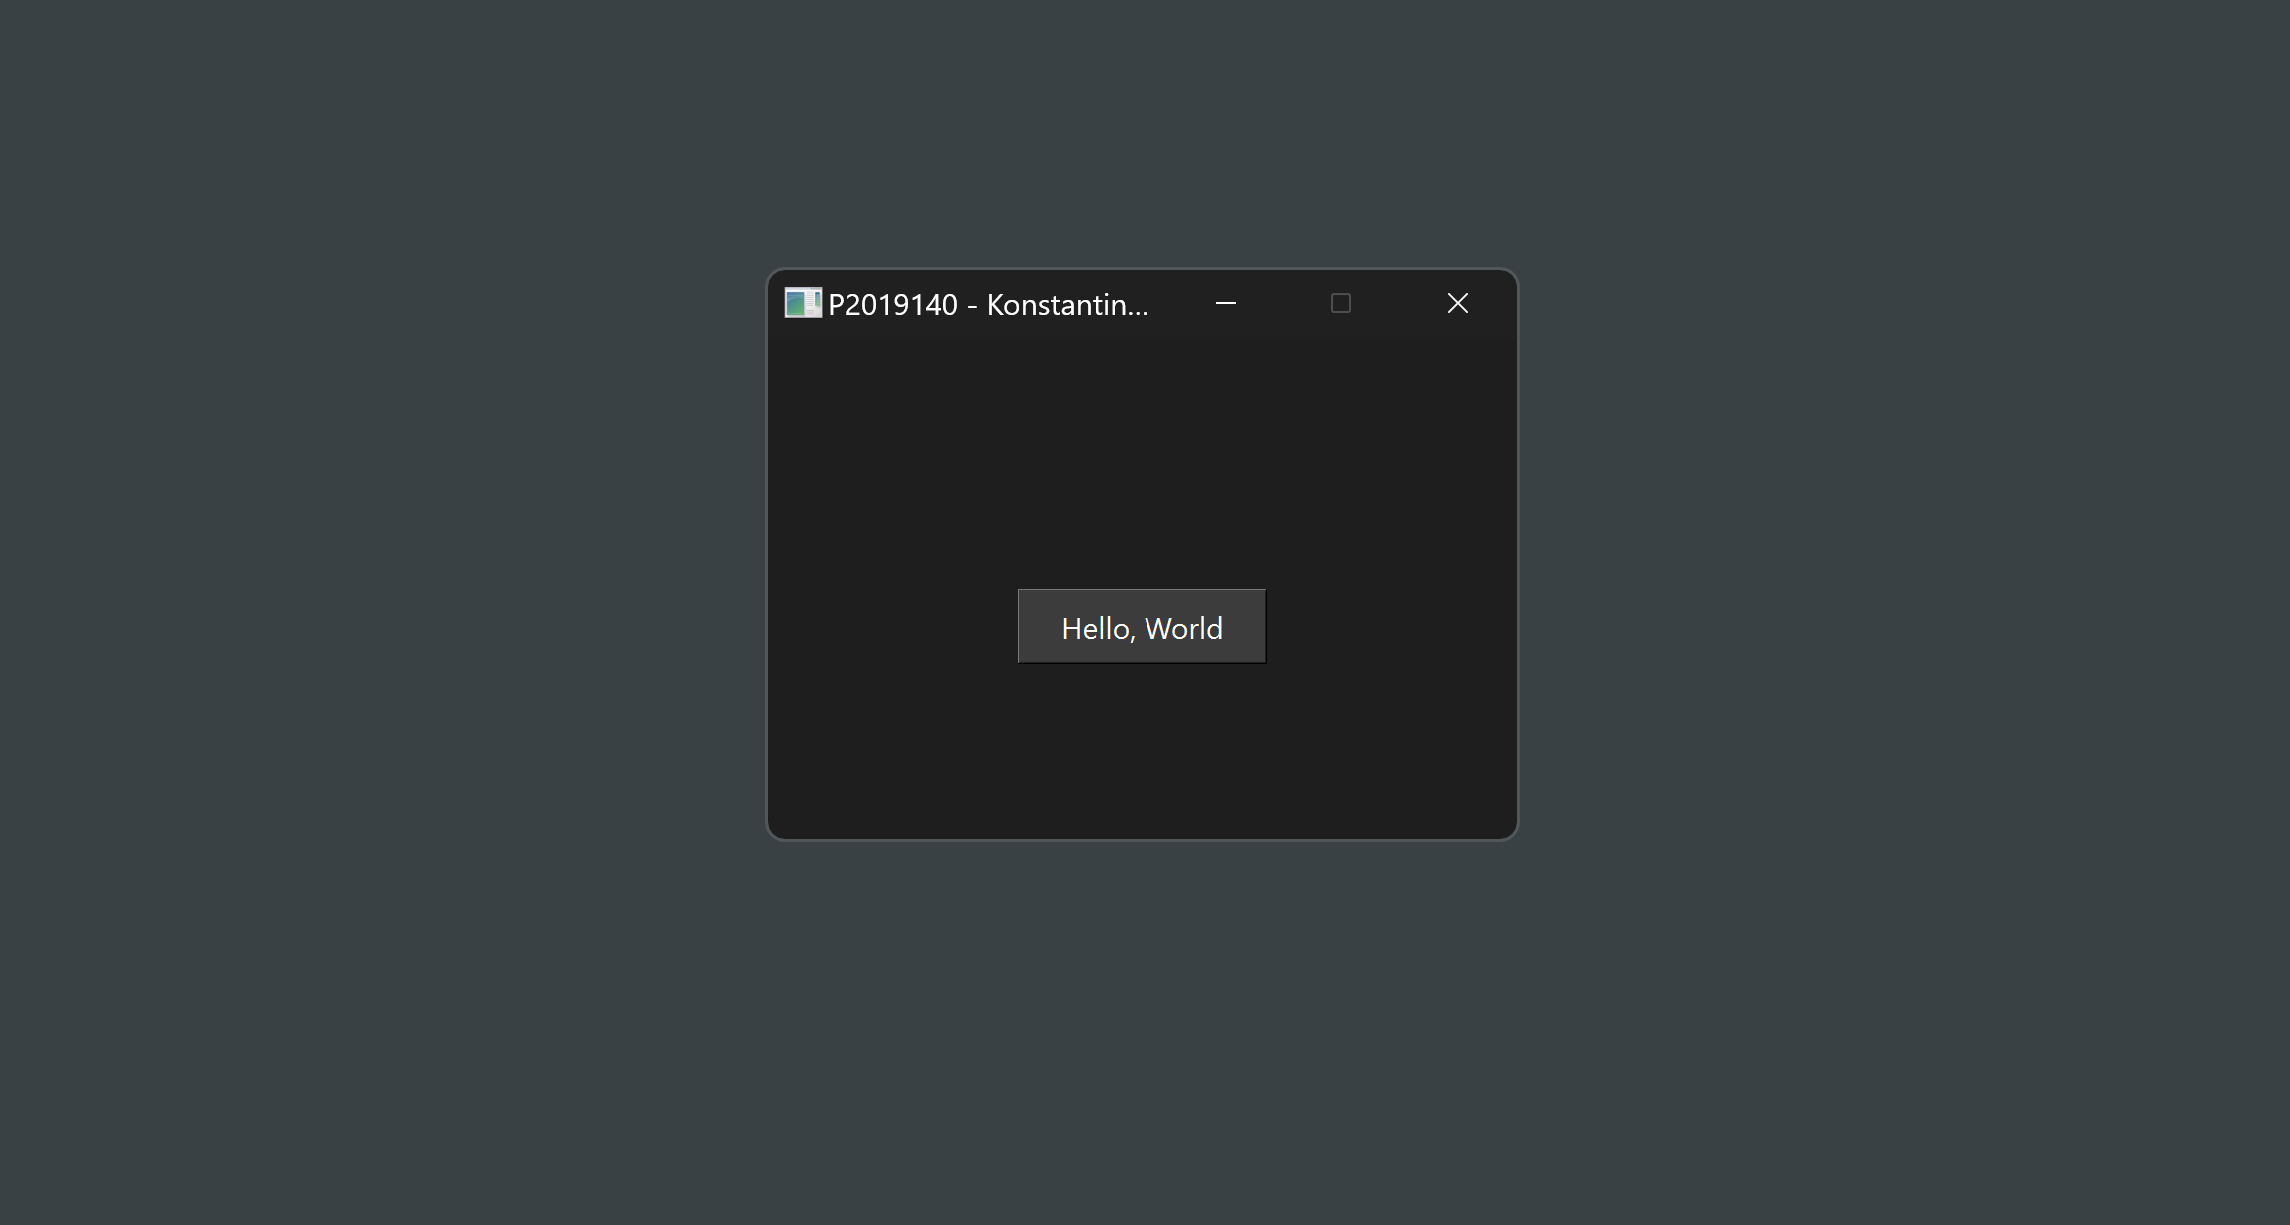
\includegraphics[width=1.0\textwidth]{./images/QPushButton.png}
    \caption{Παράθυρο Qt6 με κουμπί Hello World}
\end{figure}


Στο παράδειγμα γίνεται ή δημιουργία και ή αρχικοποίηση κουμπιού με το όνομά του και στην συνέχεια η σύνδεση.
Στην σύνδεση καλείται η μέθοδος \textbf{connect} στην οποία ορίζεται το signal το οποίο
θα πυροδοτήσει την κλήση του slot που έχει ανατεθεί στο αντικείμενο. Στην προκειμένη περίπτωση έχουμε
ορίσει το QPushButton::clicked signal το οποίο συνδέει το κουμπί με την μέθοδο PrintHello.

\subsection{Δημιουργία γραφικού πλαισίου}
Ένα layout είναι ένα πλαίσιο στο οποίο μπορούν να τοποθετηθούν άλλα στοιχεία του Qt, όπως
το QPushButton που προαναφέρθηκε. Το Qt6 παρέχει 3 βασικά είδη layouts. Το \textbf{QVBoxLayout}[4], το
\textbf{QHBoxLayout}[5] και το \textbf{QGridLayout}[6]. Τα πρώτα δύο παρέχουν ένα παρόμοιο πλαίσιο με την μόνη
τους διαφορά να βρίσκεται στην κατεύθυνση των στοιχείων μέσα στο πλαίσιο. Επομένως, ένα
QVBoxLayout χρησιμοποιείται για στοιχεία που θα τοποθετηθούν κάθετα (vertical) και ένα
QHBoxLayout θα χρησιμοποιηθεί για στοιχεία που πρόκειται να τοποθετηθούν οριζόντια (horizontal).
Τέλος, ένα QGridLayout χρησιμοποιείται για την τοποθέτηση στοιχείων σε μορφή πίνακα. Το
πλαίσιο αυτό διαθέτει θέσεις που αναπαριστούν ένα σημείο σε έναν δισδιάστατο χώρο. Κάθε σημείο
έχει μια θέση η οποία είναι μοναδική και είναι προσβάσιμη μέσω της τιμής της σειράς και της
στήλης στην οποία βρίσκεται. Παρακάτω βλέπουμε κώδικα με την χρήση ενός QVBoxLayout και την
προσθήκη ενός QPushButton σε αυτό.
\begin{lstlisting}[language=C++, style=cppstyle]
	MyWidget(QWidget *parent = nullptr) : QWidget(parent) 
    {
        setFixedSize(300, 200);
        setWindowTitle("P2019140 - Konstantinos Tourtsakis");
        
        QVBoxLayout *layout = new QVBoxLayout(this);

        QPushButton *button = new QPushButton("Hello, World", this);
        button->setGeometry(100, 100, 100, 30);

        layout->addWidget(button);

        connect(button, &QPushButton::clicked, this, &MyWidget::PrintHello);
    }

\end{lstlisting}


\begin{figure}[H]
    \centering
    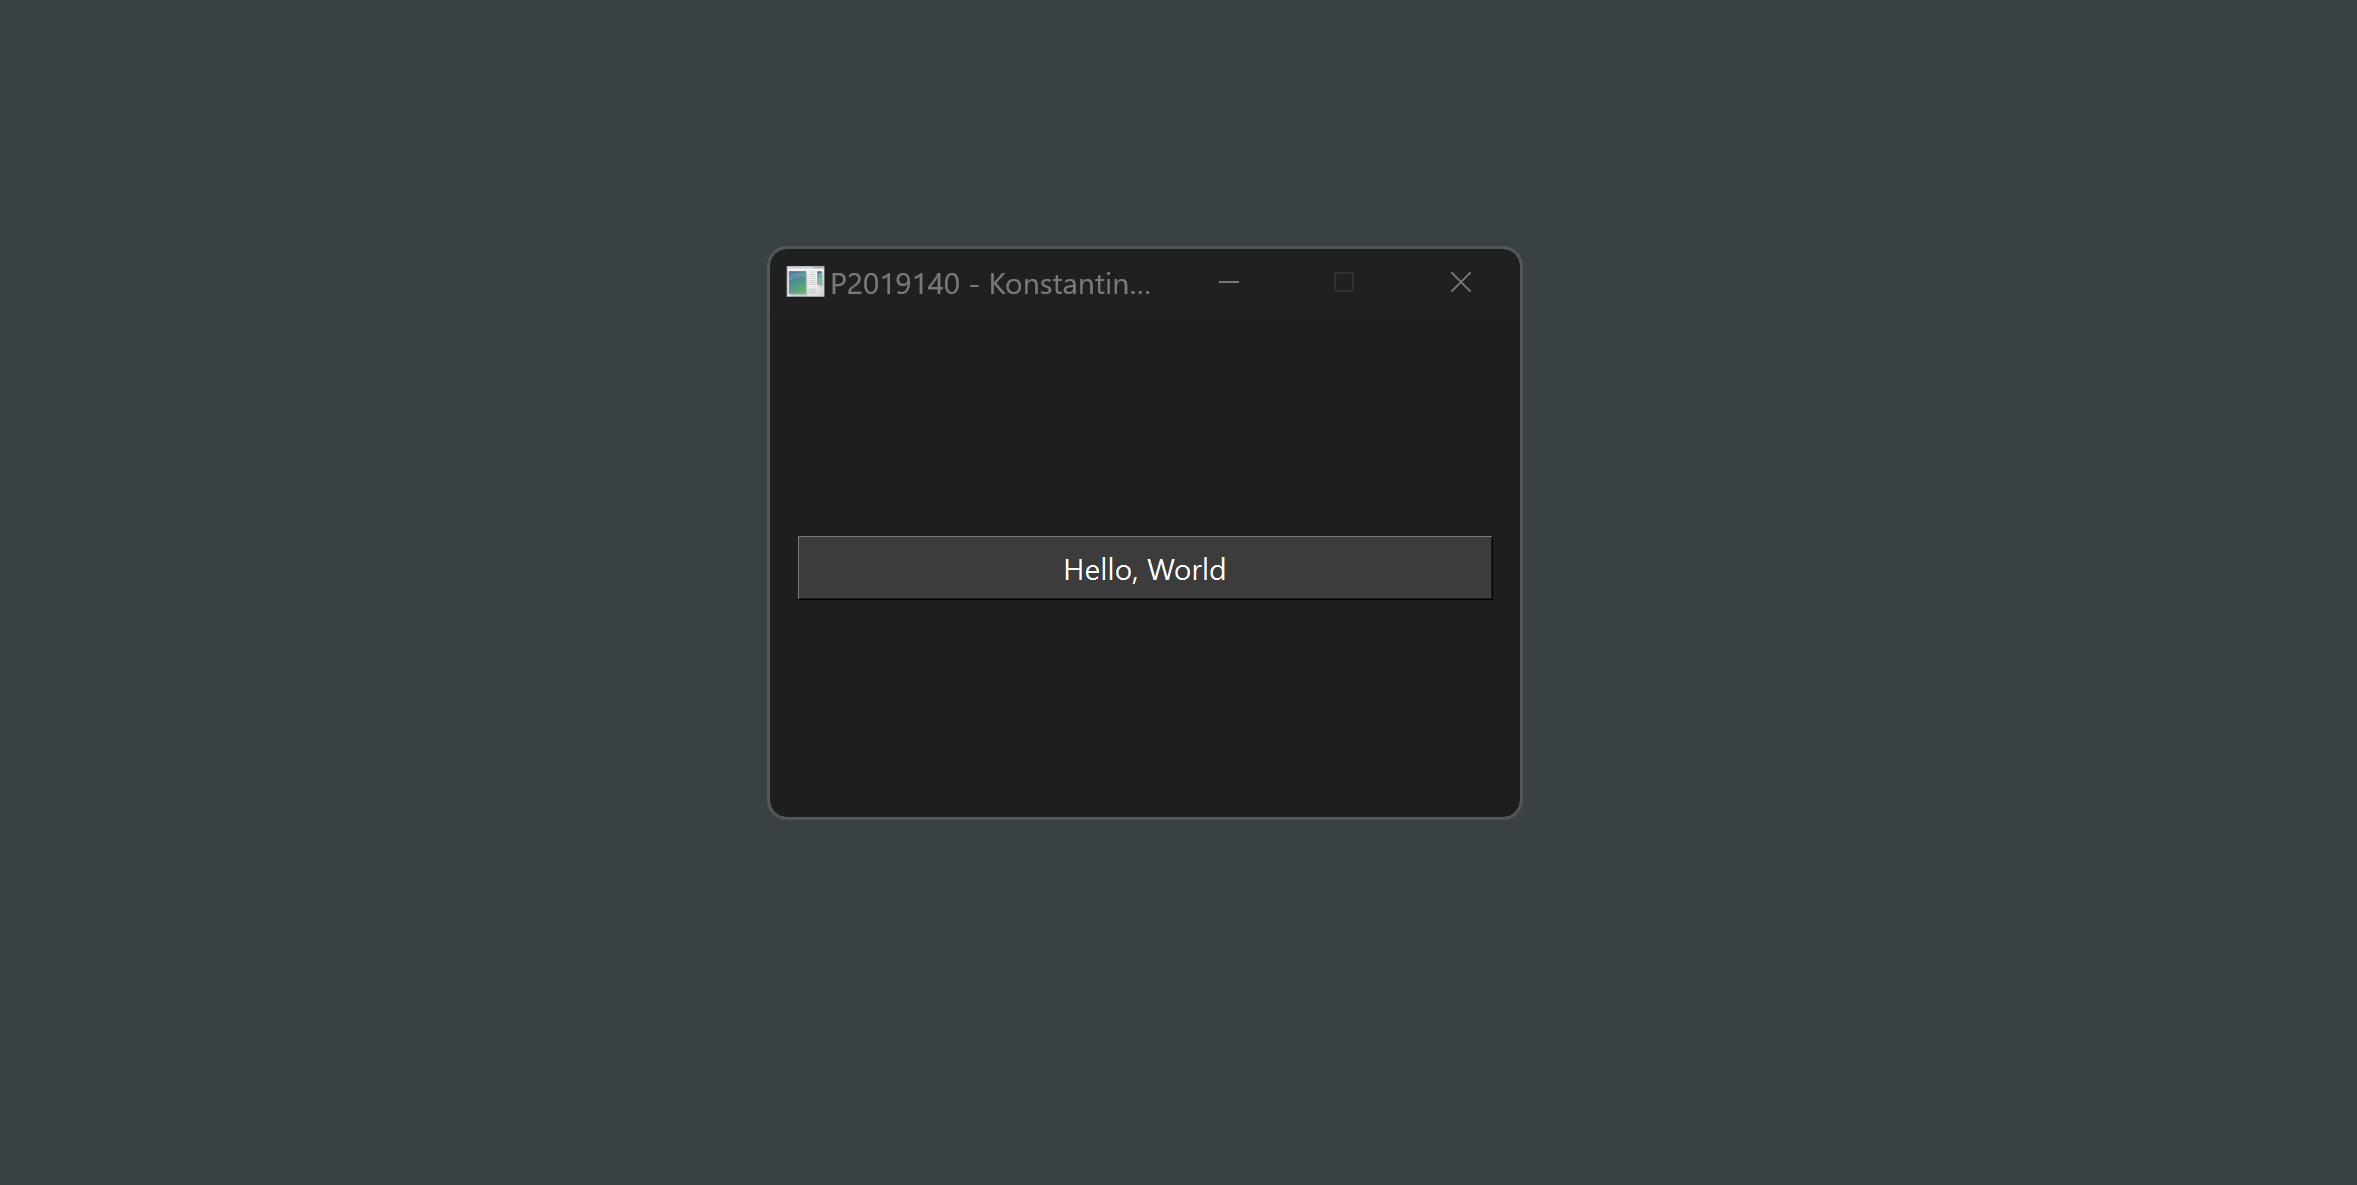
\includegraphics[width=1.0\textwidth]{./images/QVBoxLayout.png}
    \caption{Παράθυρο με κουμπί Hello World που προστέθηκε σε πλαίσιο}
\end{figure}


Κάθε στοιχείο τύπου QWidget προστίθεται πάνω στο layout με την κλήση της μεθόδου
\textbf{addWidget} και αντίστοιχα η αφαίρεση του γίνεται με την μέθοδο \textbf{removeWidget}.

\subsection{Δημιουργία λίστας αντικειμένων}
Μια λίστα QListWidget[7] μπορεί να αποθηκεύσει στην μνήμη στοιχεία τύπου QListWidgetItem.
Τα στοιχεία αυτά είναι αντικείμενα του Qt τα οποία αποθηκεύουν δεδομένα σε κάθε στοιχείο
τους και στην συνέχεια προορίζονται για προβολή των δεδομένων αυτών στη γραφική διεπαφή.
Αυτή ακριβώς είναι και η διαφορά τους με τις απλές λίστες του Qt οι οποίες δεν μπορούν να
αποτελέσουν άμεσα κομμάτι της γραφικής διεπαφής. 


\begin{lstlisting}[language=C++, style=cppstyle]
#include <QListWidget>
#include <QListWidgetItem>


class MyWidget : public QWidget 
{
public:
    MyWidget(QWidget *parent = nullptr) : QWidget(parent) 
    {
        setFixedSize(400, 300);
        setWindowTitle("P2019140 - Konstantinos Tourtsakis");

        QListWidget *list_widget = new QListWidget(this);
        list_widget->addItem(new QListWidgetItem("Item 1"));
        list_widget->addItem(new QListWidgetItem("Item 2"));
        list_widget->addItem(new QListWidgetItem("Item 3"));
        list_widget->addItem(new QListWidgetItem("Item 4"));
        list_widget->addItem(new QListWidgetItem("Item 5"));
        list_widget->setGeometry(10, 10, 200, 200);
    }
};
\end{lstlisting}


\begin{figure}[H]
    \centering
    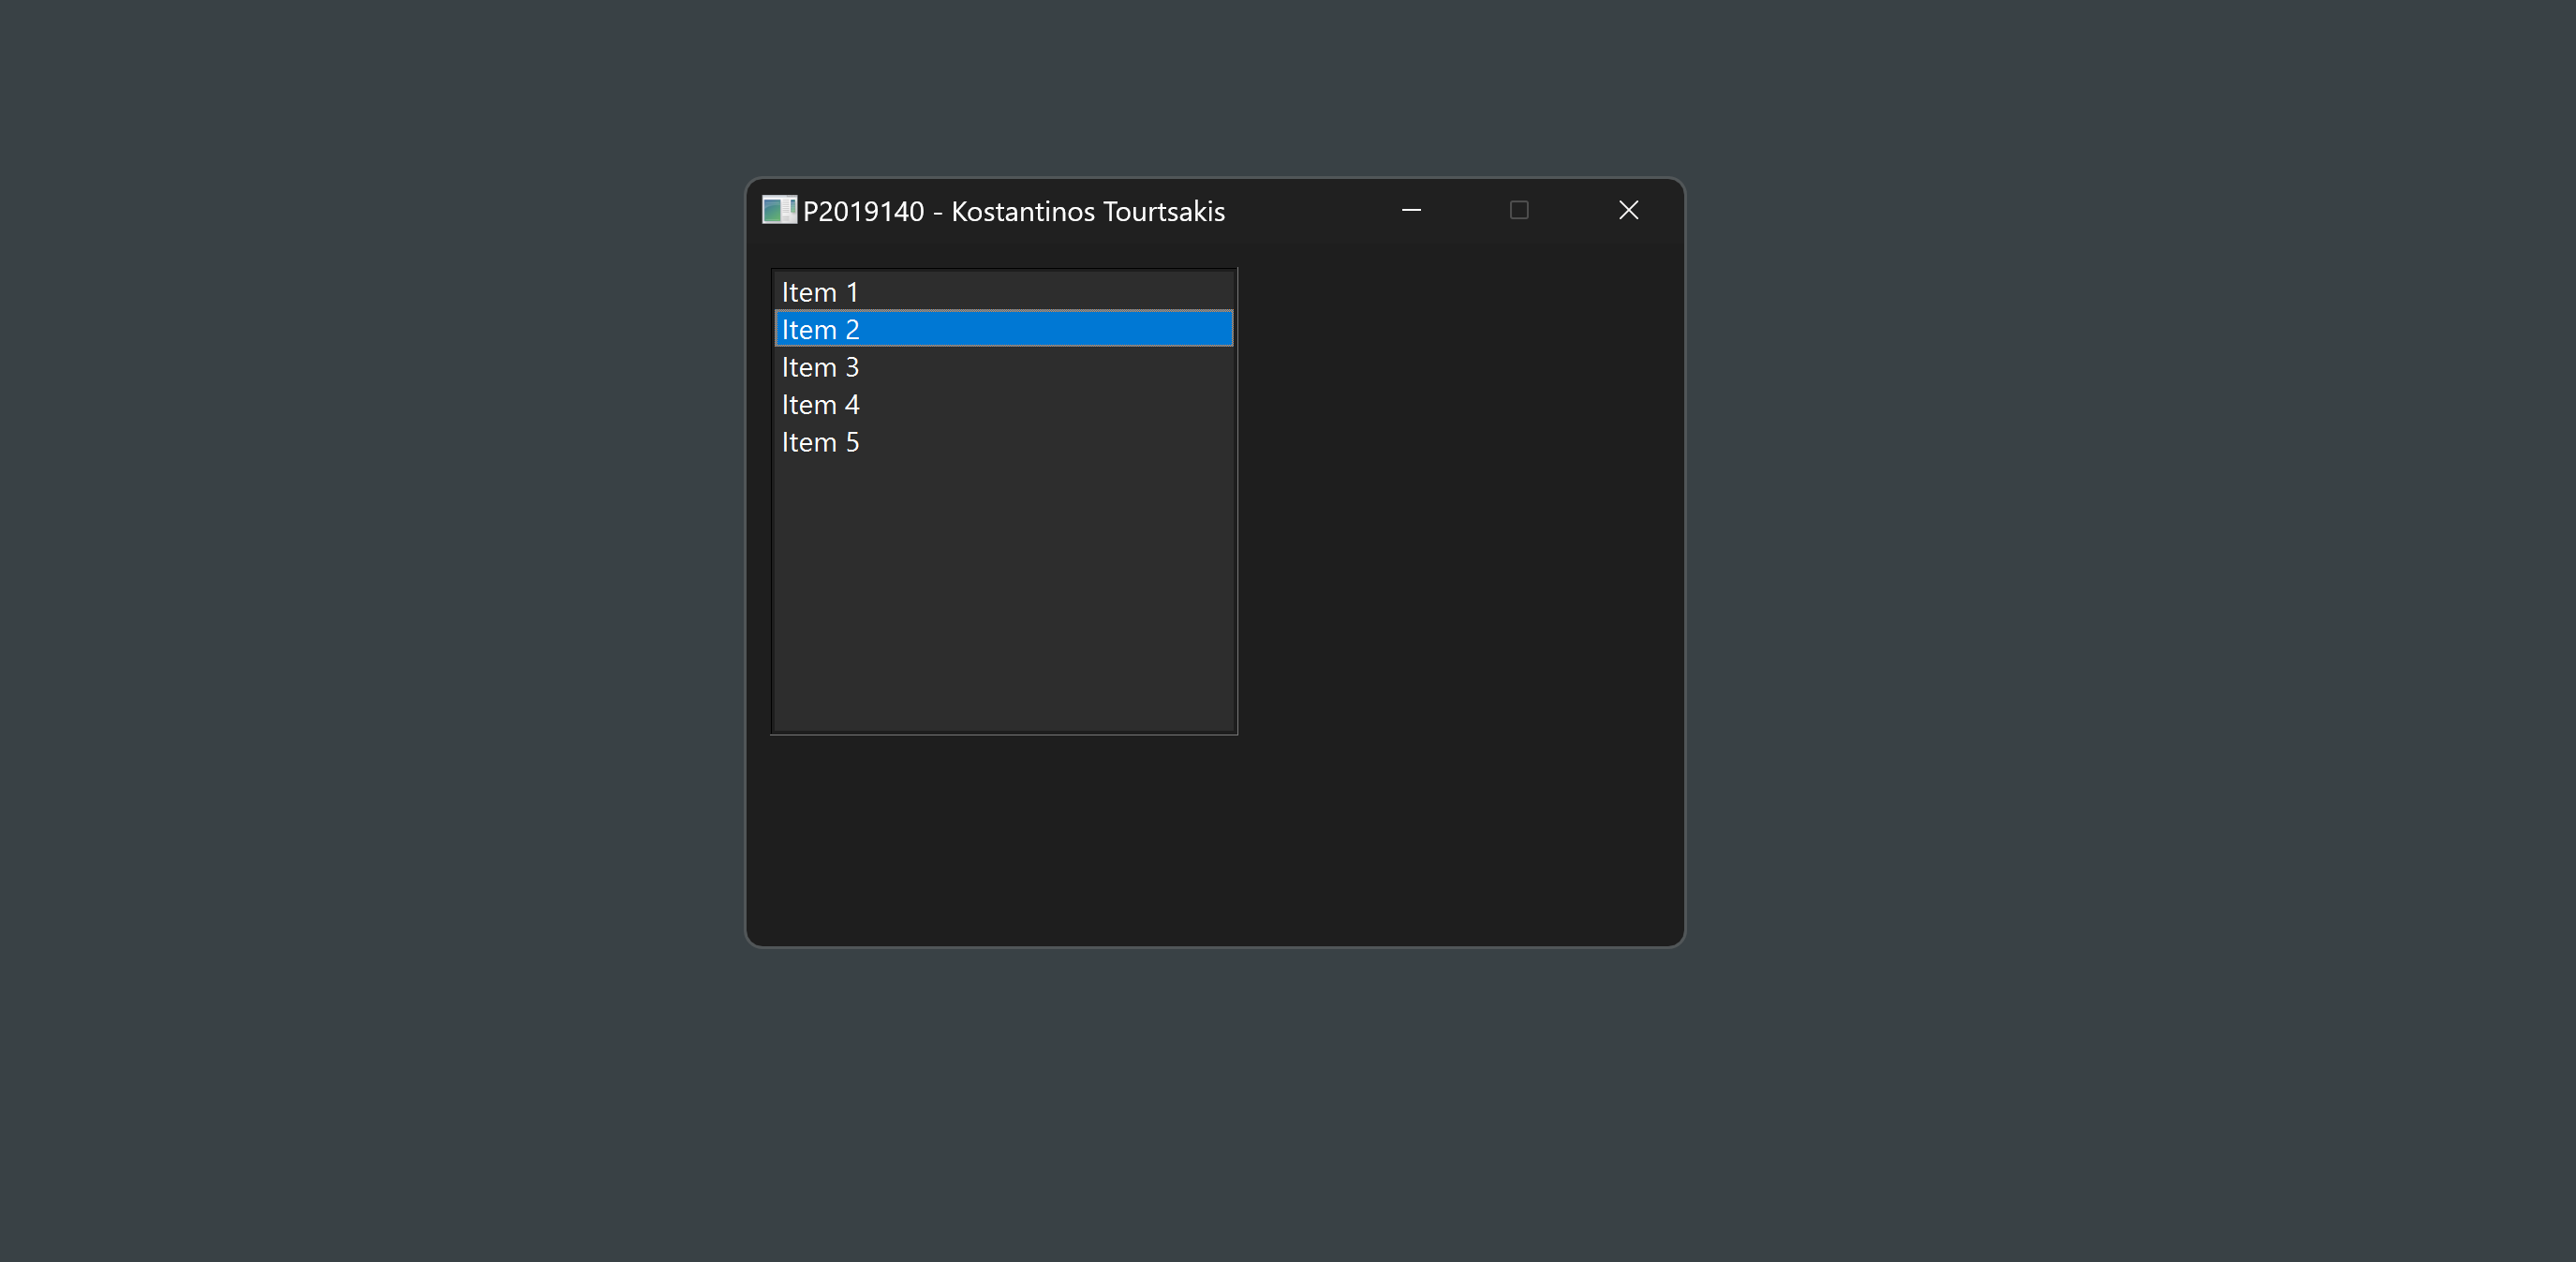
\includegraphics[width=1.0\textwidth]{./images/QListWidget.png}
    \caption{Παράθυρο Qt6 που προβάλει μια λίστα στοιχείων}
\end{figure}


\subsection{Διάβασμα αρχείων από directory}
Το διάβασμα αρχείων από ένα directory γίνεται μέσω της QDir[8] κλάσης στην οποία
αρχικοποιείται ένα αντικείμενο με το path του directory του οποίου θέλουμε να
διαβάσουμε. Στην συνέχεια αποθηκεύουμε τα ονόματα των αρχείων του directory σε μια λίστα
από QStrings την οποία διατρέχουμε για την προσθήκη τους σε ένα QListWidget
με στόχο την προβολή τους στον χρήστη.
\begin{lstlisting}[language=C++, style=cppstyle]
#include <QDir>
#include <QStringList>


class MyWidget : public QWidget 
{
public:
    MyWidget(QWidget* parent = nullptr) : QWidget(parent) 
    {
        setFixedSize(300, 200);
        setWindowTitle("P2019140 - Konstantinos Tourtsakis");

        QVBoxLayout* layout = new QVBoxLayout(this);
        QListWidget* list_widget = new QListWidget(this);
        layout->addWidget(listWidget);

        QDir directory("C:\\Users\\kosta\\Documents\\Git\\Thesis\\source\\x64\\Debug");

        QStringList files = directory.entryList(QDir::Files);
        for (const QString& file : files) 
        {
            list_widget->addItem(file);
        }
    }
};
\end{lstlisting}


\begin{figure}[H]
    \centering
    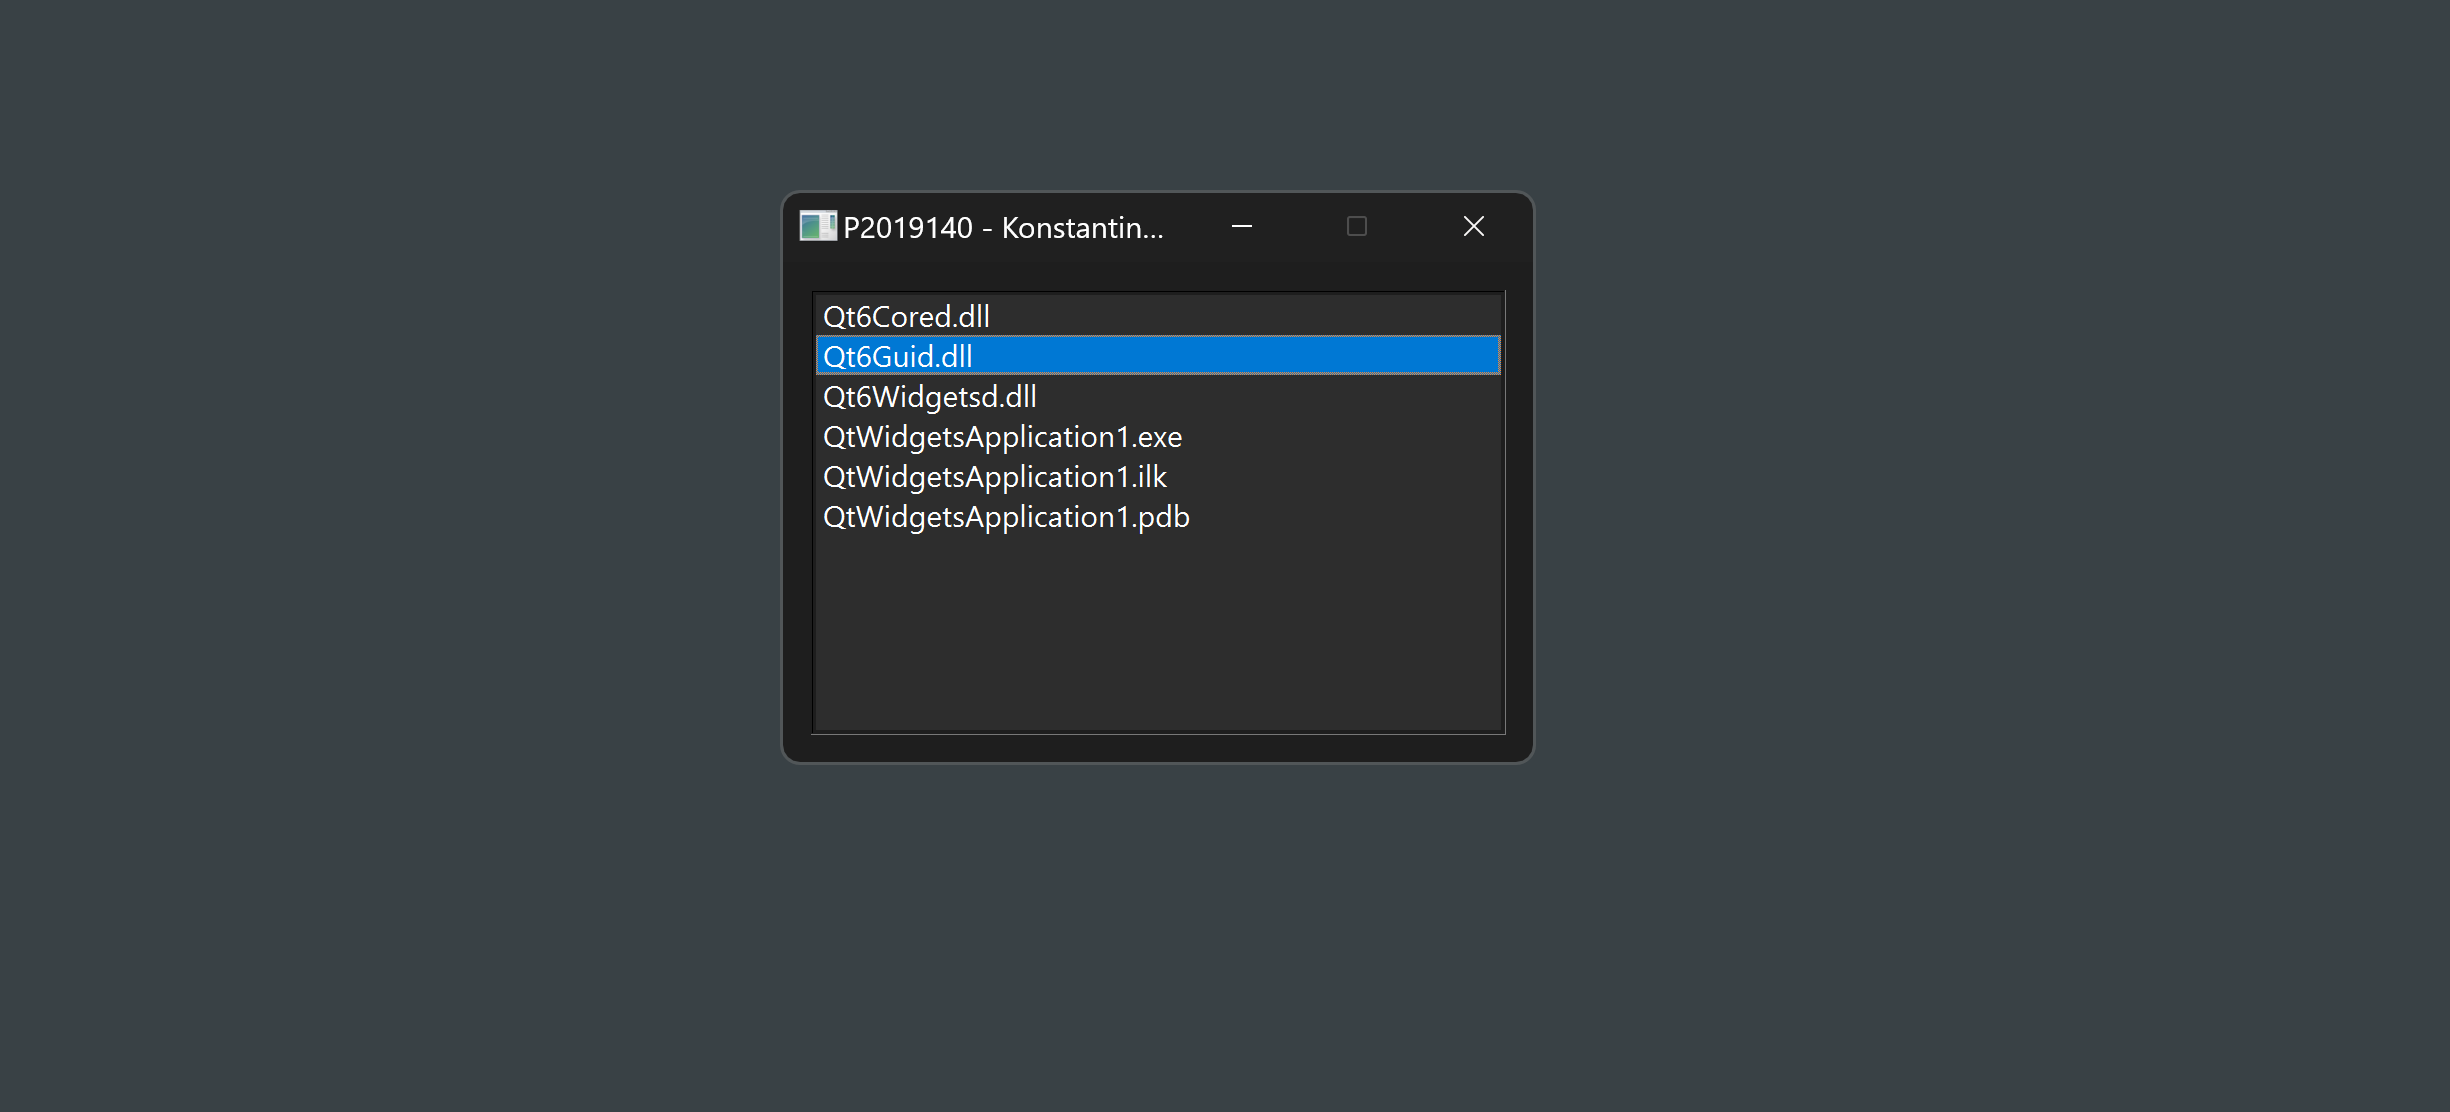
\includegraphics[width=1.0\textwidth]{./images/QDir_file_reading.png}
    \caption{Προβολή αρχείων σε λίστα}
\end{figure}


\subsection{Δημιουργία input field}
Βασικό στοιχείο κάθε εφαρμογής γραφικής διεπαφής αποτελεί το input field μιας
και επιτρέπει στον χρήστη να πληκτρολογήσει δεδομένα εισόδου για την εκτέλεση
μιας λειτουργίας του προγράμματος. Για τον σκοπό αυτό το Qt παρέχει τα αντικείμενα
τύπου QLineEdit[9]. Όπως και τα QPushButton, τα αντικείμενα αυτά αρχικοποιούνται
και στην συνέχεια προστίθενται πάνω σε ένα πλαίσιο μέσω της μεθόδου addWidget.


\begin{lstlisting}[language=C++, style=cppstyle]
#include <QLineEdit>

class MyWidget : public QWidget 
{
public:
    MyWidget(QWidget* parent = nullptr) : QWidget(parent) 
    {
        setFixedSize(400, 300);
        setWindowTitle("P2019140 - Konstantinos Tourtsakis");

        QLineEdit* lineEdit = new QLineEdit(this);
        lineEdit->setPlaceholderText("Your input goes here");
        
        QVBoxLayout* layout = new QVBoxLayout(this);
        layout->addWidget(lineEdit);

        setLayout(layout);
    }
};
\end{lstlisting}


\begin{figure}[H]
    \centering
    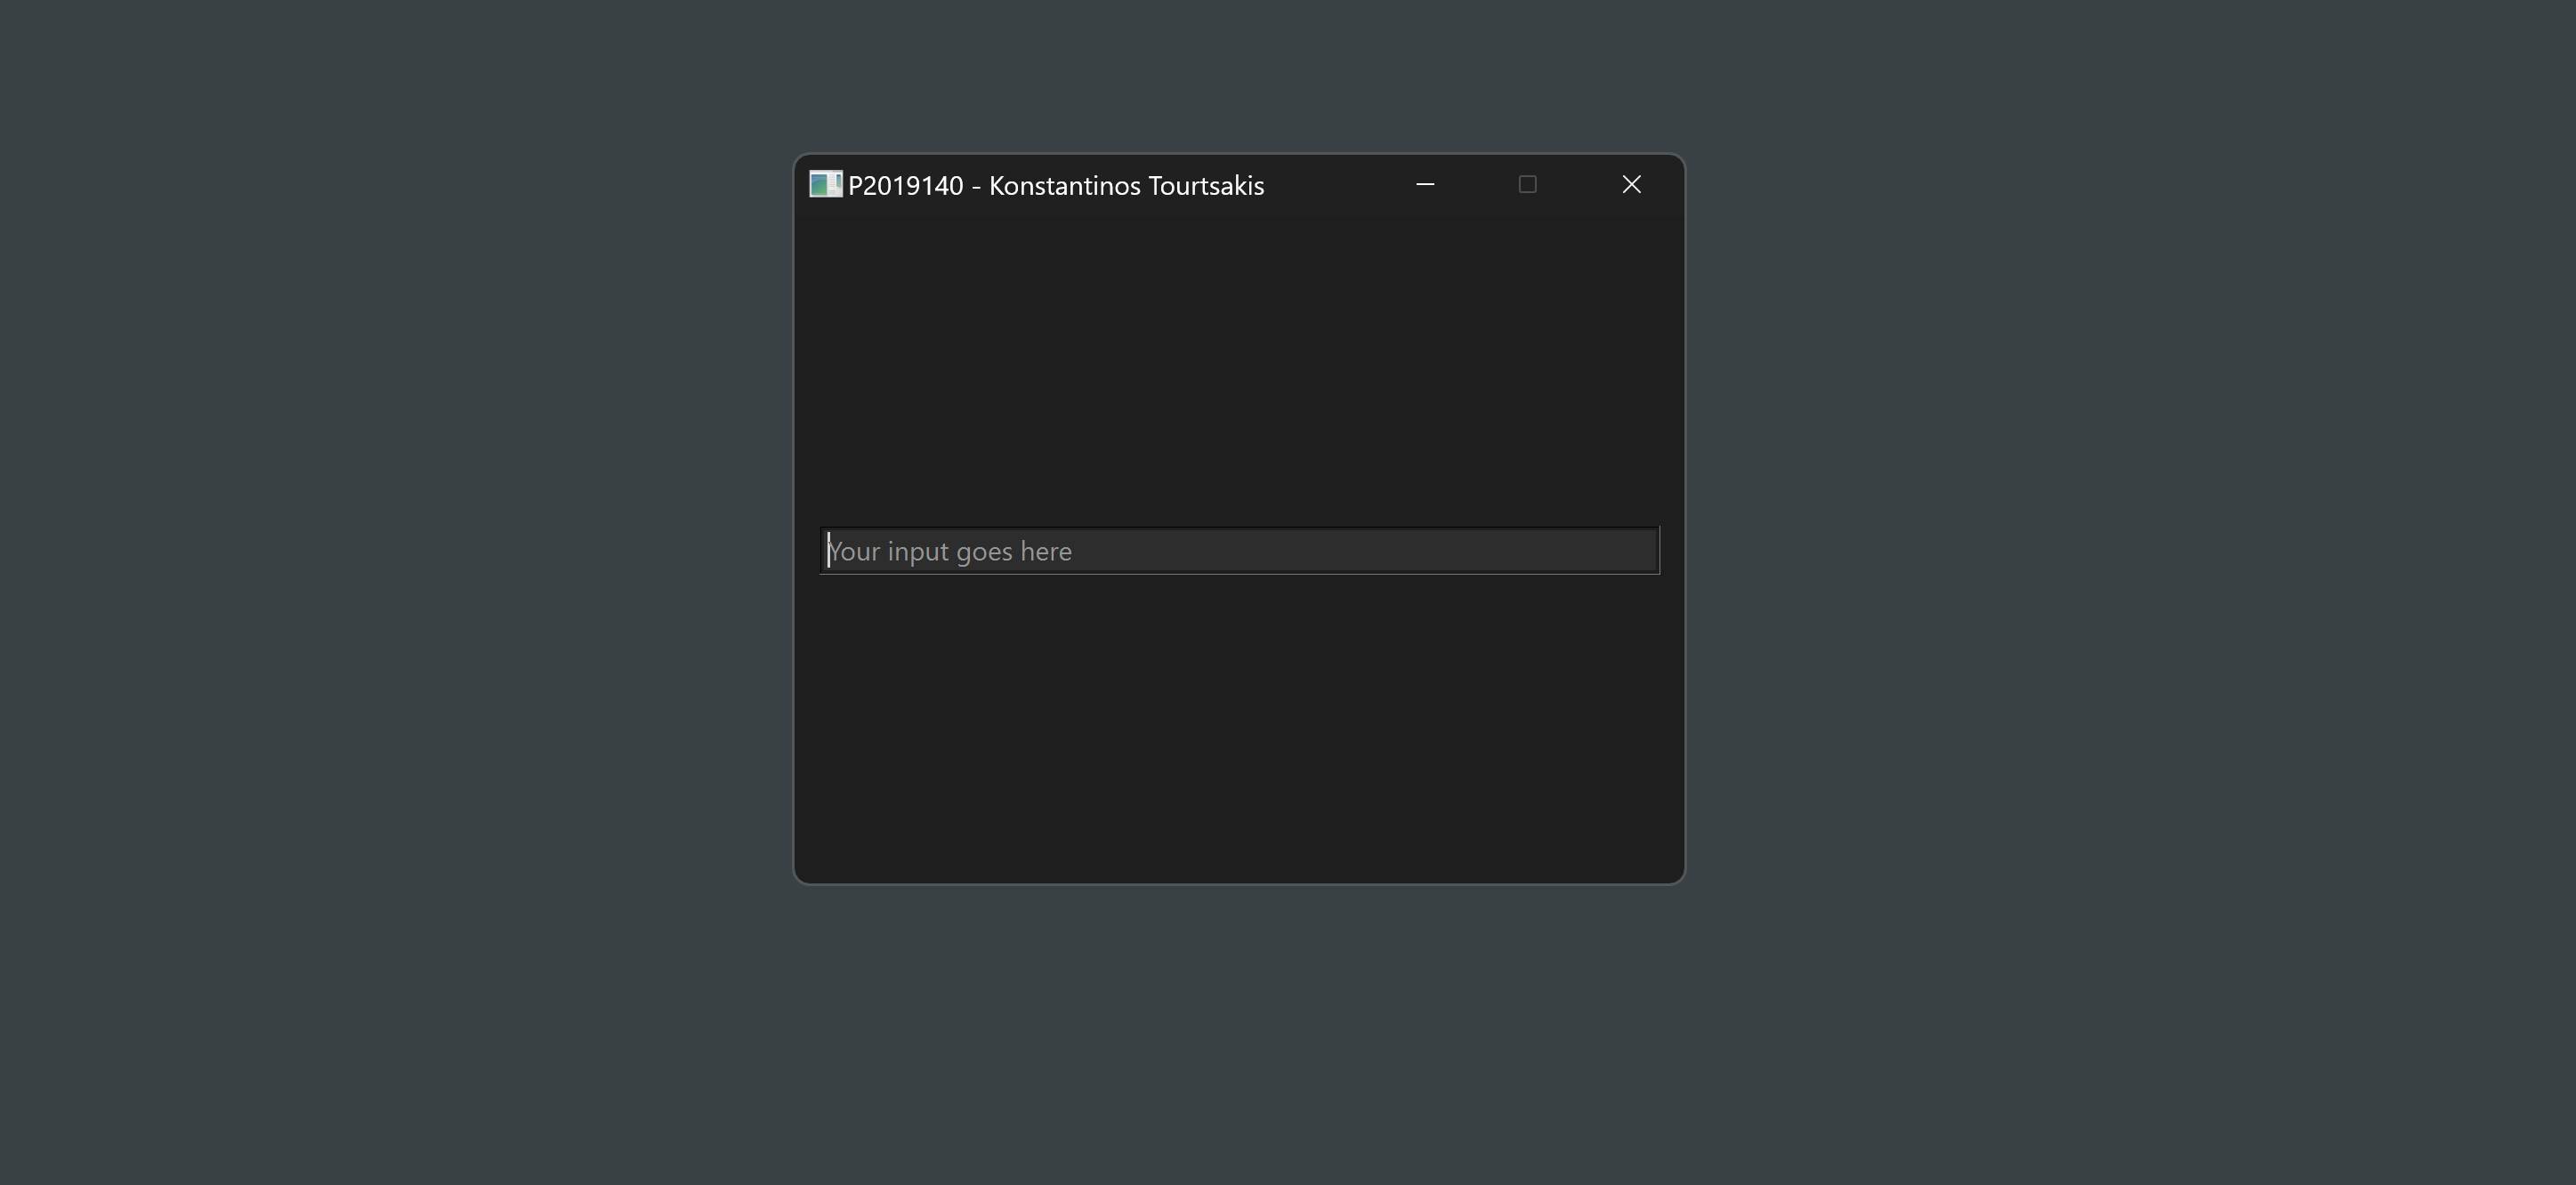
\includegraphics[width=1.0\textwidth]{./images/QLineEdit.png}
    \caption{Input field σε παράθυρο Qt6}
\end{figure}



\section{Αποθήκευση στοιχείων στον δίσκο}
Κάθε εφαρμογή στις ημέρες μας χρειάζεται να αποθηκεύει την κατάσταση στην οποία
βρισκόταν την τελευταία φορά που εκτελέστηκε με στόχο να γίνει πιο κατανοητή η
χρήση της από τον χρήστη που περιμένει να την βρει στην ίδια κατάσταση που την
άφησε όταν επιστρέψει. Για τον σκοπό αυτόν, το Qt φροντίζει να παρέχει τα απαραίτητα εργαλεία
για την αποθήκευση των στοιχείων της εφαρμογής βελτιώνοντας με αυτόν τον τρόπο
τον πηγαίο κώδικα που γράφεται για την προσθήκη της λειτουργίας αυτής. Παρακάτω
βλέπουμε μια μέθοδο που αποθηκεύει τα στοιχεία ενός Qt6 προγράμματος.


\begin{lstlisting}[language=C++, style=cppstyle]
void SaveSettings()
{
    QSettings settings("Company_name", "Application_title");
    settings.beginGroup("group_name");

    settings.setValue("WindowSize", window()->size());
    settings.setValue("Username", "JohnDoe");

    settings.endGroup("group_name");
}

\end{lstlisting}
Αρχικά δημιουργείται ένα αντικείμενο τύπου \textbf{QSettings}[10]. Ακολουθεί ο ορισμός
της ομάδας στην οποία θα γίνουν οι αλλαγές και στην συνέχεια ορίζονται
οι τιμές πάνω στις οποίες θα γραφούν οι μεταβλητές του προγράμματος. Στο τέλος
τερματίζει με το όνομα της ομάδας καλώντας την μέθοδο \textbf{endGroup}.

\section{Ανάκτηση εικονιδίων συστήματος αρχείων}
Όπως είναι γνωστό τα γραφικά περιβάλλοντα στηρίζονται πολύ στη χρήση εικονιδίων
για τη διευκόλυνση του χρήστη κατά την περιήγησή του εφόσον είναι πολύ πιο
αποτελεσματική η συσχέτιση μιας λειτουργίας με μια εικόνα παρά με κάποιο κείμενο.
Επομένως, είναι σημαντικό να υπάρχει στην εφαρμογή μια συνάρτηση που επιστρέφει το εικονίδιο
ενός αρχείου δυναμικά, έτσι ώστε ο χρήστης να καταλαβαίνει από την αρχή τη λειτουργία που
κρύβεται πίσω από την ενεργοποίηση του εικονιδίου αυτού. Παρακάτω βλέπουμε την συνάρτηση αυτή.


\begin{lstlisting}[language=C++, style=cppstyle]
QIcon GetFileIcon(const QString& file_path)
{
    SHFILEINFO shfi;
    memset(&shfi, 0, sizeof(SHFILEINFO));

    if (SHGetFileInfo(reinterpret_cast<const wchar_t*>(file_path.utf16()), 0, &shfi, sizeof(SHFILEINFO), SHGFI_ICON | SHGFI_USEFILEATTRIBUTES))
    {
        QPixmap pixmap = QPixmap::fromImage(QImage::fromHICON(shfi.hIcon)).scaled(QSize(PercentToWidth(6.66), PercentToHeight(11.85)), Qt::KeepAspectRatio, Qt::SmoothTransformation);
        QIcon icon(pixmap);

        // Cleanup the icon resource
        DestroyIcon(shfi.hIcon);

        return icon;
    }

    
    return QIcon();
}
\end{lstlisting}

Επειδή η εφαρμογή στην οποία αναφέρεται το παρόν κείμενο προορίζεται για χρήση σε
συστήματα Windows, η συγκεκριμένη συνάρτηση στηρίζεται πάνω σε αυτά. Αρχικά
δημιουργείται ένα struct τύπου SHFILEINFO πάνω στο οποίο θα αποθηκευτούν τα
δεδομένα του αρχείου, συμπεριλαμβανομένου και του εικονιδίου. Στη συνέχεια γίνεται
έλεγχος για την ανάκτηση του εικονιδίου από το σύστημα. Αφού η ανάκτηση γίνει με
επιτυχία, δημιουργείται ένα \textbf{QPixmap} με το εικονίδιο του αρχείου. Στη 
συνέχεια το pixmap χρησιμοποιείται για τη δημιουργία του QIcon[11][12] εικονιδίου το
οποίο και θα επιστραφεί από τη συνάρτηση. Αν το εικονίδιο ενός αρχείου δεν ανακτηθεί, 
η συνάρτηση θα επιστρέψει ένα προεπιλεγμένο QIcon.


\section{Προτάσεις δεδομένων εισόδου σε input field}

Συχνά οι χρήστες βρίσκουν χρήσιμη την υποβοήθησή τους από τη γραφική διεπαφή
στην περιήγησή τους στο εκάστοτε πρόγραμμα. Μια τέτοια βοήθεια μπορεί να παρασχεθεί
επίσης κατά την είσοδο δεδομένων σε ένα input field. Ανάλογα με τις ενέργειες του
χρήστη υπάρχει κάποιος αλγόριθμος που καθορίζει τη λίστα από την οποία το
input field θα προτείνει στον χρήστη δεδομένα εισόδου. Στο Qt αυτή η λειτουργία
υλοποιείται με ένα αντικείμενο QCompleter[13] που ουσιαστικά συμπληρώνει αυτό που έχει
γράψει ο χρήστης με προτάσεις δεδομένων.

\begin{lstlisting}[language=C++, style=cppstyle]
    QLineEdit input_field;
    QStringList suggestions;
    suggestions << "Suggestions" << "for" << "thesis";
    
    QCompleter* completer = new QCompleter(suggestions, &input_field);
    completer->setCaseSensitivity(Qt::CaseInsensitive);
    
    input_field.setCompleter(completer);
\end{lstlisting}



\section{Επαναληπτική εκτέλεση διεργασιών παρασκηνίου}

Ένα βασικό πρόβλημα με τις βιβλιοθήκες εφαρμογών γραφικής διεπαφής είναι το γεγονός
πως αμέσως μετά την δημιουργία των γραφικών στοιχείων η βιβλιοθήκη αποκτά τον πλήρη
έλεγχο της εφαρμογής με αποτέλεσμα να μην είναι εφικτή η εκτέλεση κώδικα επαναληπτικά.
Αυτό καθιστά αδύνατη την εκτέλεση διεργασιών ρουτίνας οι οποίες πρέπει να εκτελούνται
σε κάθε επανάληψη του προγράμματος ώστε να γίνει εφικτή η υλοποίηση ορισμένων λειτουργιών.
Ευτυχώς οι περισσότερες βιβλιοθήκες, όπως και το Qt, διαθέτουν αντικείμενα που επιτρέπουν
την προσθήκη κώδικα που εκτελείται σε τακτά χρονικά διαστήματα τα οποία ορίζονται από τον
προγραμματιστή. Αυτό όπως είναι κατανοητό μπορεί να αξιοποιηθεί ορίζοντας ένα μηδενικό
χρονικό διάστημα, δημιουργώντας κατά κάποιο τρόπο μια επανάληψη που την διαχειρίζεται το
Qt[14].

 \begin{lstlisting}[language=C++, style=cppstyle]
QTimer* timer = new QTimer(this);
connect(timer, &QTimer::timeout, this, &MyWidget::TaskMainUserLoop);
timer->start(0);
\end{lstlisting}

